% % % Document Type
% % % Ref.: http://www.biwako.shiga-u.ac.jp/sensei/kumazawa/tex/book.html
%\documentclass[11pt, a4paper, openany]{book}

% % Recommendation: pdflatex

% % For xelatex, https://www.overleaf.com/project/65a713928bbe39eb0faab35apdflatex, and lualatex, please use the documentclass as bellow:
\documentclass[12pt, a4paper, openany]{book}


% % For platex, please use the documentclass as below:
%\documentclass[12pt, a4paper, openany, dvipdfmx]{book}


% % % 
% For Overleaf users:
% You can use Overleaf to write your thesis.
% If you use `` platex '' compiler, you must see the below link which is the Overleaf document for platex:
% https://ja.overleaf.com/learn/latex/Questions/Does_Overleaf_support_pTeX%3F
% Then if you can not compile your project with platex compiler, please downgrade the compiler version to 2020 or 2019.


% If any errors occur, please try to fix the errors.


% % % Necessary
\usepackage{amssymb, amsmath, latexsym}  % For mathematics [Before hyperref]
\usepackage[setpagesize=false]{hyperref} % For inserting hyperlink [Before graphicx]
\usepackage{graphicx}                    % For inserting figure
\usepackage{subcaption}                  % For caption of figures and tables
\usepackage[usenames]{color}             % For coloring
\usepackage[shortlabels]{enumitem}       % For useful enumerate and itemize environment
\usepackage{comment}                     % For commenting multiline
\usepackage{cite}                        % For citing references [After hyperref]
\usepackage{url}                         % For inserting URL
\usepackage{acro}                        % For listing abbreviations and symbols
\usepackage{master}                      % For master thesis [After graphicx and color]

% % % Convenient for tables and emphasis
\usepackage{tabularx}       % For flexible table
\usepackage{multirow}       % For combining multi rows for table
\usepackage{colortbl}       % For coloring table
\usepackage{longtable}      % For long table across multiple pages
\usepackage[normalem]{ulem} % For flexible underline etc.
\usepackage{bxascmac}       % For framing multiline
\usepackage{graphicx}
% % % Option
\usepackage{siunitx}   % For using SI units
\usepackage{afterpage} % For inserting newpage
\usepackage{listings}  % For inserting programming code
\usepackage{docmute}   % For compilation of divided files

% % % Configuration for hyperlink
\hypersetup{ %
	breaklinks=true, %
	colorlinks=false, %
	urlcolor=blue, %
	urlbordercolor={0 1 1}}

% % % Define Command
\newcommand{\bm}[1]{\mbox{\boldmath $#1$}}

% % % Re-define names

% % 論文題目     / Title
\title{Photorealistic 3D virtual environment for robot navigation and manipulation using neural radiation fields and Unreal Engine 5}
% % 著者名       / Author name
\author{Yuminosuke Sato}
% % 修了時期     / Year and month when you complete master course
\datestamp{March 2024} 
% % 主査名と職階 / Name and position of chief examiner
\mainreferee{Yuichi Yagichi}    
\mainrefereeposition{Senior Associate Professor}
% % 副査名と職階 / Name and position of deputy examiner
\secondreferee{Keitaro Naruse }
\secondrefereeposition{Professor}
\thirdreferee{Watanobe Yutaka}
\thirdrefereeposition{Associate Professor}

% % You can define abbreviations and symbols, if any.
% % If you show lists of either abbreviations, symbols or both, 
% % you should define them in ./Chapter/Acronym.tex
% % However, if you do not need the lists, you should comment out the following line
% % and replace \showlist command to \showlists{y}{y}{n}{n}
% % % Reference: 
% http://tex.stackexchange.com/questions/86666/how-to-create-both-list-of-abbreviations-and-list-of-nomenclature-using-nomencl
% ftp://ftp.kddilabs.jp/CTAN/macros/latex/contrib/acro/acro_en.pdf
% % %
\usepackage{acro}
% Configuration for hyperlink and list of acronyms
\acsetup{hyperref=true, list-style=longtable, list-heading=chapter*}

% class `abbrev': abbreviations:
\DeclareAcronym{pc}{
  short = PC ,
  long  = Personal Computer ,
  class = abbrev
}
\DeclareAcronym{ws}{
  short = WS ,
  long  = Work Station ,
  class = abbrev
}
\DeclareAcronym{uoa}{
  short = UoA,
  long  = University of Aizu,
  class = abbrev
}

% class `nomencl': nomenclature (symbol)
\DeclareAcronym{A}{
  short = $\bm{A}$ ,
  long  = Matrix ,
  sort  = A ,
  class = nomencl
}
\DeclareAcronym{a}{
  short = $\bm{a}$ ,
  long  = Vector ,
  sort  = a ,
  class = nomencl
}
\DeclareAcronym{r}{
  short = $\mathbb{R}$ ,
  long  = Set of real numbers ,
  sort  = R ,
  class = nomencl
}



\begin{document}
% % タイトル、著作権、承認ページ、目次の作成 
% % Make pages for title, copyright, approval and table of contents
\makefrontmattar

% % 図、表、略語、記号一覧の表示
% % Show lists of figures, tables, abbreviations and symbols (Optional)
% % %
% % If you set 'n' to the fourth argument of \showlists{figures}{tables}{abbreviaions}{symbols}
% % (i.e. \showlists{y}{y}{y}{n}), list of symbols is not shown.
% % Similarly, you can decide if you show each list. 
% % %
\showlists{y}{y}{y}{y}
% \showlists{y}{y}{n}{n}

% % 謝辞を挿入 / Acknowledment (Optional)
\chapter*{Acknowledgment}
% % 要旨を挿入
\chapter*{Abstract}
To address the challenge of bridging the gap between virtual and real-world environments in robotics, this study proposes an innovative approach that leverages Luma AI's Neural Radiance Fields (NeRF) and Unreal Engine 5 (UE5). The study uses standard smartphone cameras to capture video footage and efficiently create photorealistic 3D virtual environments. These environments are then integrated with UE5 to simulate realistic robotic navigation and manipulation tasks. The method's effectiveness is validated through objective evaluations using Navigation2 for operational efficacy and YOLO for accurate object recognition in both virtual and real settings. The study demonstrates a significant reduction in the time and resources required for environment creation compared to existing methods like NeRF2real and Matterport3D. This advancement facilitates simulation-driven development and testing in robotics and establishes a new standard for virtual environment generation. 
\thispagestyle{empty}


% % %
% Begin of Body
% % %
\configbody

% % When you request examiners to do peer review of your thesis, the paper should be double-spacing.
% % When you submit your thesis, the paper must be single-spacing.
\singlespacing
% \doublespacing

% % Chapterごとにファイルを分けて,それぞれをincludeする
% % You should make files of each chapter, and include them.
% % docmute package is convenient to edit and compile each file. If you are interested, please search the package.
\chapter{Introduction}
\label{chap:introduction}
\begin{table}[h]
    \caption{Comparison of functions of common robot simulators \cite{collins2021review}}
    \centering
    \renewcommand{\arraystretch}{1.5}
    \setlength{\extrarowheight}{5pt}
    \resizebox{\textwidth}{!}{% 
        \large % 文字の大きさを大きくする
        \begin{tabular}{|c|c|c|c|c|c|c|c|c|c|c|c|c|c|}
        \hline Simulator & \begin{tabular}{c} 
        RGBD \\
        + \\
        LiDAR
        \end{tabular} & \begin{tabular}{l} 
        Force \\
        Sensor
        \end{tabular} & \begin{tabular}{c} 
        Linear + Cable \\
        Actuator
        \end{tabular} & \begin{tabular}{l} 
        Multi-Body \\
        Import
        \end{tabular} & \begin{tabular}{l} 
        Soft-Body \\
        Contacts
        \end{tabular} & \begin{tabular}{c} 
        DEM \\
        Simulation
        \end{tabular} & \begin{tabular}{c} 
        Fluid \\
        Mechanics
        \end{tabular} & \begin{tabular}{l} 
        Headless \\
        Mode
        \end{tabular} & \begin{tabular}{c} 
        ROS \\
        Support
        \end{tabular} & HITL & Teleoperation & \begin{tabular}{c} 
        Realistic \\
        Rendering
        \end{tabular} & \begin{tabular}{c} 
        Inverse \\
        Kinematics
        \end{tabular} \\
        \hline Airsim & $\checkmark$ & \times & \times & \times & \times & \times & \times & $\checkmark$ & $\checkmark$ & $\checkmark$ & $\checkmark$ & $\checkmark$, unreal & \times \\
        \hline CARLA & $\checkmark$ & \times & \times & \times & \times & \times & \times & $\checkmark$ & $\checkmark$ & \times & $\checkmark$ & $\checkmark$, unreal & \times \\
        \hline CoppeliaSim & $\checkmark$ & $\checkmark$ & \begin{tabular}{l} 
        Linear \\
        only
        \end{tabular} & $\checkmark$ & \times & $\checkmark$ & \times & $\checkmark$ & $\checkmark$ & $\checkmark$ & $\checkmark$ & \times & $\checkmark$ \\
        \hline Gazebo & $\checkmark$ & $\checkmark$ & \begin{tabular}{l} 
        Linear \\
        only
        \end{tabular} & $\checkmark$ & \times & \begin{tabular}{l} 
        Through \\
        Fluidix
        \end{tabular} & \begin{tabular}{l} 
        Through \\
        Fluidix
        \end{tabular} & $\checkmark$ & $\checkmark$ & $\checkmark$ & $\checkmark$ & \times & $\checkmark$ \\
        \hline MjoCo & $\checkmark$ & $\checkmark$ & $\checkmark$ & $\checkmark$ & $\checkmark$ & $\checkmark$ & Limited & $\checkmark$ & \times & \begin{tabular}{l} 
        HAPTIX \\
        only
        \end{tabular} & \begin{tabular}{l} 
        HAPTIX \\
        only
        \end{tabular} & \times & \times \\
        \hline PyBullet & $\checkmark$ & $\checkmark$ & \begin{tabular}{l} 
        Linear \\
        only
        \end{tabular} & $\checkmark$ & $\checkmark$ & $\checkmark$ & \times & $\checkmark$ & \times & \times & $\checkmark$ & \times & $\checkmark$ \\
        \hline SOFA & \times & \times & $\checkmark$ & $\checkmark$ & $\checkmark$ & $\checkmark$ & $\checkmark$ & $\checkmark$ & $\checkmark$ & $\checkmark$ & $\checkmark$ & $\checkmark$, Unity & \times \\
        \hline UWSim & \begin{tabular}{l} 
        RGBD \\
        only
        \end{tabular} & $\checkmark$ &\times & $\checkmark$ & \times & \times & \times & $\checkmark$ & $\checkmark$ & $\checkmark$ & $\checkmark$ & $\checkmark$, custom & \times \\
        \hline Chrono & $\checkmark$ & $\checkmark$ & $\checkmark$ & \times & $\checkmark$ & $\checkmark$ & $\checkmark$ & $\checkmark$ & \times & \times & $\checkmark$ & $\checkmark$, offline & $\checkmark$ \\
        \hline Webots & $\checkmark$ & $\checkmark$ & linear & $\checkmark$ & \times & \times & Limited & $\checkmark$ & $\checkmark$ & \times & $\checkmark$ & \times & \times \\
        \hline
        \end{tabular}
    }
    \label{tab:Comparisonoffunctionsofcommonrobotsimulators}
\end{table}

\singlespacing
In the realm of robotics, overcoming the disparity between simulated environments and real-world applications presents a significant hurdle\cite{anderson2021sim}. The creation of a simulation environment inherently presupposes its congruence with the actual world, a notion fraught with complexity. Integrating real-world physical limitations within such a simulated framework is notably challenging\cite{Acosta2021Validating,Miglino1995Evolving}. Acknowledging and surmounting this divergence is imperative for the advancement and societal integration of robotic technologies.
\singlespacing

Several robot simulation environments have been proposed to integrate simulations with the physical limitations of the real world \cite{collins2021review}.  There are various simulation environments for robots(shown in Table.\ref{tab:Comparisonoffunctionsofcommonrobotsimulators}). For example, Gazebo\cite{koenig2004design} and Choreonoid\cite{nakaoka2012choreonoid} for service robots. Unity\cite{unity2023}, Unreal Engine 4\cite{unrealengine4}, and 5\cite{unreal2023engine} for general arm robots. There are several simulation environments available for different applications, such as AirSim\cite{shah2018airsim}, FlightGear\cite{sorton2005simulated}, and CARLA. It is important to use specific terms consistently and adhere to industry standards for metrics and units. Additionally, there are system simulation environments, like air traffic control, that do not require a physical environment.  These robotics simulation environments integrate real-world physical limitations.
\singlespacing

Robotic simulation environments pose challenges in accurately replicating large 3D spaces. For example, those used by service robots. Creating 3D virtual environments is a costly and time-consuming process, making it difficult to achieve both realism and accuracy\cite{connolly2021realistic}\cite{byravan2023nerf2real}. In the real world, objects are segmented and formed into complete shapes, with light textures and reflections from light sources appearing as continuous surfaces. In simulations, objects are represented as a sampling of discrete points, which makes it difficult to replicate the continuity of reality\cite{slater2002computer}.
\singlespacing
Accurately recreating real-world 3D environments is crucial for completing specific challenges. Importing real-world 3D environments automatically can help meet these challenges\cite{Liu2017Design}. However, in 3D virtual environments, the color representation of textures on object surfaces is not constant, which poses a major challenge. This is because textures are measured in different colors depending on the reflection of the light source. Accurate color reproduction is crucial for realistic 3D environments, as color indeterminacy affects not only visible light but also light sources like lasers. To achieve this, it is important to have a precise understanding of texture color.
\singlespacing

 We suggest a straightforward, precise, and photorealistic mapping method for constructing 3D virtual environments, along with a robot simulation system that employs it. The environment is modeled using Luma AI\cite{luma2023unreal}, a cloud-based Neural Radiance Field (NeRF)\cite{mildenhall2020nerf} technology that allows for photorealistic rendering of 3D objects. The Luma AI-generated environment model produces a 3D virtual environment and point cloud. Two maps are constructed from this point cloud: a voxel map for pathfinding and a near-visual surface map for recognition. The voxel map is used by the robot to navigate while the near-visual surface map is used for recognition.
\singlespacing

To implement the robot simulation system, we will utilize Unreal Engine 5 to create a simulation environment that closely resembles reality. The engine will display visual maps and place voxel maps as obstacles. The robot simulation will use Robot Operating System2(ROS2)\cite{ros2}, a visual map for robot recognition in visible light, and a voxel map that uses depth sensing technology for object recognition and avoidance. 
\singlespacing
This research presents pivotal advancements in the realm of robotic simulation environments, addressing the critical challenge of bridging the gap between simulated and real-world settings. Firstly, it emphasizes the integration of real-world physical limitations into simulation environments, a task previously noted for its complexity and necessity for the progress of robotic technologies. By employing specific simulation environments like Gazebo, Choreonoid, Unity, Unreal Engine 4 and 5, AirSim, FlightGear, and CARLA, this study adheres to industry standards, ensuring consistency and relevance. Furthermore, it tackles the formidable task of replicating large 3D spaces accurately, a known issue in robotic simulations, particularly for service robots. The introduction of a novel mapping method using Luma AI and Neural Radiance Field (NeRF) technology marks a significant leap forward. This method not only achieves photorealistic rendering of 3D objects but also facilitates the construction of realistic virtual environments and point clouds. The creation of dual maps from these point clouds - a voxel map for robot navigation and a near-visual surface map for recognition - represents a nuanced approach to robotic perception and interaction within these simulated environments. Lastly, the implementation of this technology in a robot simulation system using Unreal Engine 5 and ROS2 demonstrates a practical application of these theoretical advancements, showcasing a system that utilizes both visual and depth sensing technologies for enhanced robot recognition and obstacle avoidance. These contributions collectively represent a substantial stride towards more accurate, realistic, and functional robotic simulation environments, bridging the gap between simulation and real-world application, and setting a new standard for future research in this field.
\chapter{Related Work}
\label{cha:Related Work}
\section{Photorealistic scene reconstruction technology}
\label{sec:Photorealistic scene reconstruction technology}

Our approach to indoor environment modeling differs from traditional datasets. While common datasets like Matterport3D\cite{chang2017matterport3d} and Gibson\cite{xia2018gibson}, Replica\cite{straub2019replica} use custom-built scanning equipment with depth and LIDAR capabilities, we use a small number of video images from consumer-grade mobile cameras to train NeRF and model the scene. This approach is fundamentally different from other studies, such as Habitat-Matterport3D\cite{shah2018airsim}.


\section{Neural Radiance Fields in robotics}
\label{sec:Neural Radiance Fields in robotics}

NeRF has a wide range of applications in robotics. However, our research takes a different approach from previous work. NeRF has been used for posture estimation\cite{lin2021inerf}, representation learning\cite{lin2022nerf-supervision}, grasping behavior\cite{ichnowski2021dex-nerf}, and learning dynamic models\cite{driess2022learning}. Although traditional state estimation and planning methods for obstacle avoidance in simulated NeRF environments have been studied, their real-world applications remain untested. Our research will focus on creating a simulation environment for these studies.

\section{Unreal engine in robotics}
\label{sec:Unreal engine in robotics}
The Unreal Engine has been widely used in robotics research, especially in developing simulation environments. This emphasizes the engine's capability to produce immersive and authentic virtual environments for off-road autonomous driving and robotic vision \cite{young2020unreal, martinez-gonzalez2019unrealrox}. It showcases the engine's potential in creating accurate ground-truth datasets and real-time physics simulations of robotic behavior \cite{pollok2019unrealgt}. These studies highlight the Unreal Engine's adaptability and efficiency in driving forward research in robotics.
\chapter{Method}
\label{chap:Method}
\section{System Overview}
\label{sec:system_overview}

\begin{figure}[htbp]
  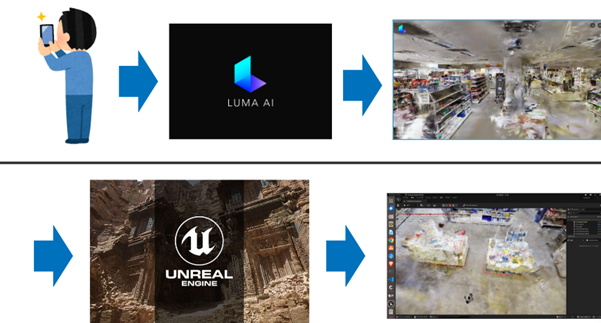
\includegraphics[scale=0.9]{./Figure/画像16.png}
  \caption{Illustration of you writing the master thesis}
  \label{fig:itai}
\end{figure}
\singlespacing
Our research encompasses the development of a three-dimensional, photorealistic environment, culminating in the comprehensive assessment of the Turtlebot3 robot's operational efficacy within this milieu (as elucidated in Figure 3.1). The initial phase entails capturing a video in a verisimilitudinous setting utilizing either an iPhone or an Android smartphone, both equipped with a monocular camera. Post-capture, this footage is uploaded to the advanced Luma AI platform for intricate processing, yielding a three-dimensional, photorealistic environment accompanied by detailed point cloud data. Subsequently, these components are integrated into the Unreal Engine 5 (UE5), facilitating the simulation of a real-world-esque, three-dimensional, photorealistic virtual habitat. Within this UE5 framework, the Turtlebot3 robot conducts a series of simultaneous photographic captures in both the virtual and the actual environments, enabling a holistic evaluation and nuanced analysis of its operational performance in both simulated and tangible real-world scenarios. This comprehensive assessment yields invaluable insights into the robot's functional prowess and its potential applicability across diverse environmental contexts.
\singlespacing
\begin{figure}[htbp]
  \centering
  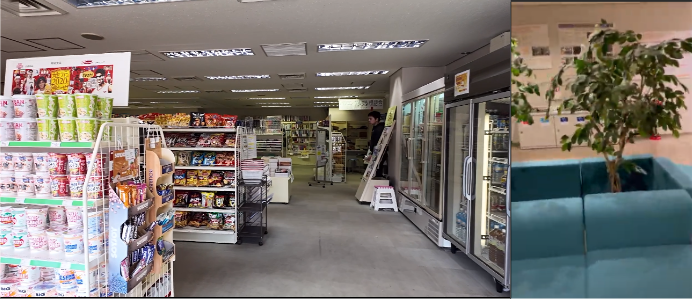
\includegraphics[scale=0.6]{./Figure/画像24.png}
  
  \caption{two real-world environments}
  \label{fig:two real-world environments}
\end{figure}
\section{Video for 3D virtual enviroments}
\label{sec:video for 3D virtual enviroments}
\singlespacing
We recreated two real-world environments as 3D virtual environments using a smartphone camera and a DJI Pocket 2. The environments include a convenience store kiosk, a university educational facility research building, and a laboratory located within the University of Aizu. Our goal was to capture the unique characteristics of each location. The environments include a convenience store kiosk, a university educational facility research building, and a laboratory located within the University of Aizu. Filming took approximately 30 minutes, and select images from each location are shown in \ref{fig:two real-world environments}.
\singlespacing
The images were captured using the iPhone 12 Pro camera and the DJI Pocket 2. The iPhone 12 Pro has three 12MP lenses with different features: ultra-wide angle, wide-angle, and telephoto lenses. The DJI Pocket 2 is a high-performance camera with a compact size and 3-axis stabilization, supporting a variety of video resolutions and modes. With these cameras, high-quality video of three real-world environments was successfully captured.



\section{Video Processing Using Luma AI}
\label{sec:Video Processing Using Luma AI}
\singlespacing
To capture a video and generate a virtual 3D space using LumaAI's NeRF technology, follow these steps:
\singlespacing
First, use your smartphone camera to record the desired environment from multiple angles.  This will provide NeRF with the necessary information to create detailed 3D models. To capture a complete picture of the environment, it is recommended to shoot in slow and steady motions.
\singlespacing
Afterwards, upload the video data to LumaAI's NeRF system, which uses deep learning to analyze the shape and position of objects, lighting conditions, and other factors from each frame in the video to reconstruct a 3D scene.
\singlespacing
After completing the process, LumaAI's NeRF generates a detailed 3D model of the captured environment. This model enables users to observe the scene from different angles, in addition to the original video perspective, allowing for free exploration of the virtual environment.


\begin{figure}[htbp]
  \centering
  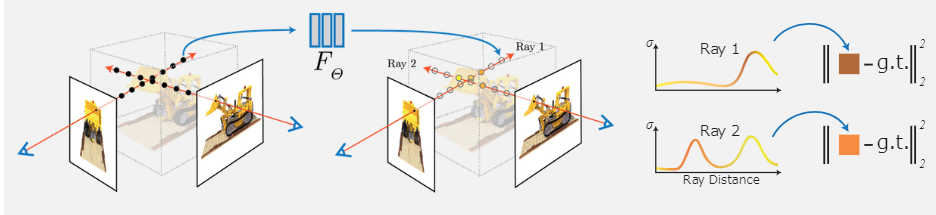
\includegraphics[scale=0.55]{./Figure/画像19.png}
  
  \caption{NeRF synthesizes images by sampling coordinates, processing through an MLP for color and density, and compositing via volume rendering, optimizing by comparing with real images.}
  \label{fig:NeRF synthesizes images}
\end{figure}


\subsection{Neural Radiance Fields (NeRF)}
\label{sec:Neural Radiance Fields (NeRF)}
\singlespacing
Neural Radiance Fields\cite{lin2021inerf}, commonly abbreviated as NeRF, represent a groundbreaking approach in the field of computer vision and 3D reconstruction. This technique, which emerged from the intersection of deep learning and computer graphics, has garnered significant attention for its ability to create highly detailed and photorealistic 3D models from a set of 2D images.
\singlespacing
At its core, NeRF is a novel way to represent 3D scenes. Traditional 3D modeling techniques, like polygon meshes or voxel grids, have limitations in terms of rendering complex details and realistic lighting effects. NeRF addresses these limitations by using a fully connected deep neural network to model the volumetric scene. Essentially, it learns a continuous representation of the scene, mapping spatial coordinates and viewing directions to color and density values. This mapping is achieved through a process called volume rendering, which integrates the contributions of light along a ray passing through the scene(shown in \ref{fig:NeRF synthesizes images}).
\singlespacing
One of the most striking features of NeRF is its ability to synthesize novel views of a scene with high fidelity. Given a set of 2D images taken from different viewpoints, NeRF can interpolate and extrapolate from this data to generate new images from perspectives not originally captured. This is particularly valuable in applications like virtual reality, where immersive experiences depend on realistic and fluid rendering of 3D environments.
The training process of a NeRF model involves optimizing the neural network to minimize the difference between the rendered images and the actual input photographs. This optimization is computationally intensive, as it requires processing thousands of rays through the neural network to accurately capture the light interactions in the scene. However, the results are often stunning, with NeRF models capable of capturing intricate details like reflections, refractions, and complex lighting conditions that are challenging for traditional 3D modeling methods.
\singlespacing
NeRF's applications extend beyond just creating photorealistic renderings. It's also being explored in fields like cultural heritage preservation, where it can be used to create detailed digital replicas of historical artifacts or sites from a limited number of photographs. In robotics and autonomous vehicles, NeRF can assist in creating detailed 3D maps of environments. In the film and entertainment industry, it offers new possibilities for visual effects and virtual production, allowing for seamless integration of virtual and real elements.
\singlespacing
Despite its impressive capabilities, NeRF does have some limitations. The computational resources required for training and rendering are significant, which can be a barrier to real-time applications. Additionally, the quality of the output heavily depends on the quantity and quality of the input images. Scenes with highly dynamic elements or transparent objects still pose challenges for NeRF models.
\singlespacing
In conclusion, Neural Radiance Fields represent a significant advancement in 3D scene representation and rendering. By leveraging the power of deep learning, NeRF offers a way to create highly detailed and realistic 3D models from ordinary photographs. Its potential applications are vast, spanning various industries, and it continues to be an active area of research, with ongoing efforts to overcome its current limitations and expand its capabilities.
\singlespacing
\begin{figure}[htbp]
  \centering
  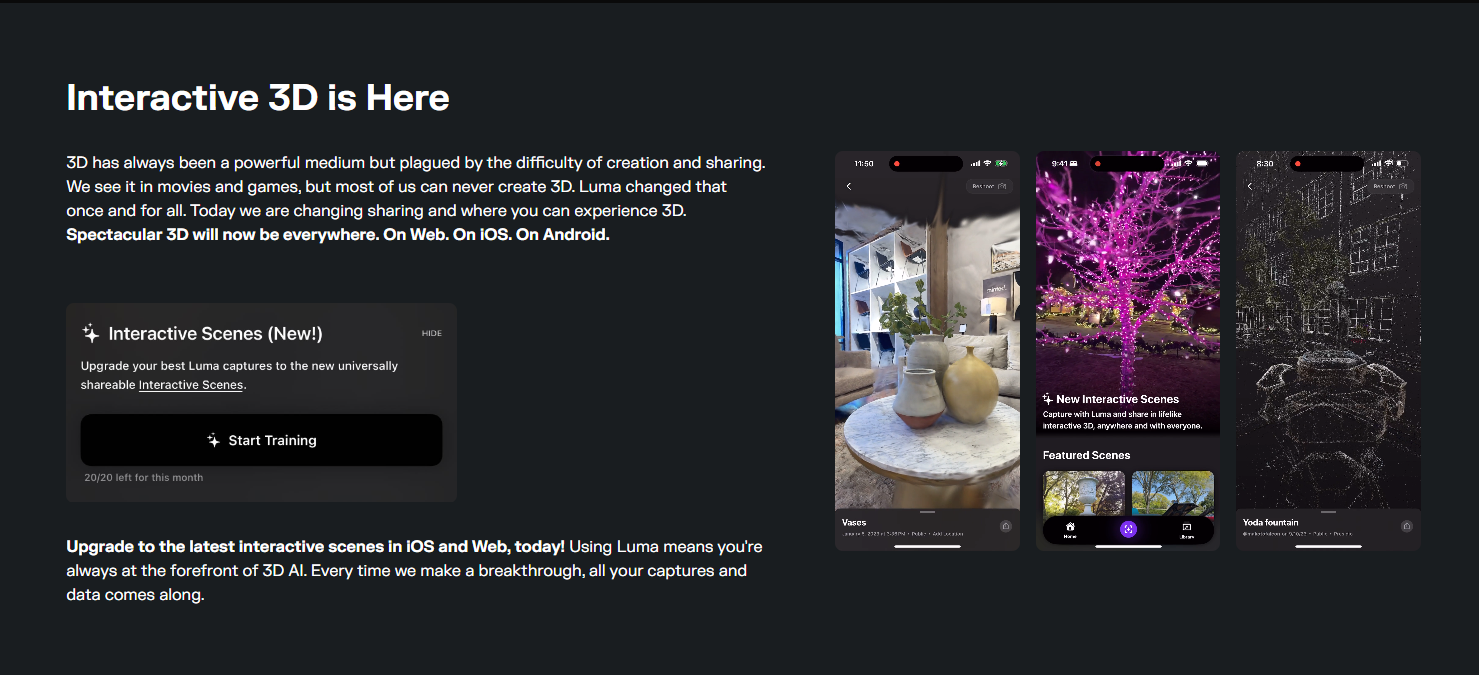
\includegraphics[scale=0.35]{./Figure/画像20.png}
  \caption{Luma AI Platform site}
  \label{fig:Luma AI Platform site}
\end{figure}
\subsection{Luma AI Platform}
\label{sec:Luma AI Platform}
\singlespacing
Luma AI\cite{lumaai} is an innovative scanning application capable of capturing objects in three dimensions. This app stands out for its ability to generate and output precise 3D models, available in both a web version and an iOS version. Users can create 3D models by uploading videos or capturing real objects using a smartphone camera. Notably, Luma AI utilizes NeRF (Neural Radiance Fields) technology, which reconstructs three-dimensional states through machine learning using multiple photographs.
\singlespacing
Delving into the usage of this app, one must first set up an account, followed by capturing the object from various angles through filming or photography. After uploading these videos or photos to Luma AI(see.\ref{fig:Luma AI Platform site}), the AI employs this data to generate a highly detailed 3D model of the targeted object. These models can be converted into various formats such as GLTF, OBJ, or USDZ, offering flexibility in usage. By default, captures are set to private, but options are available to share them publicly with the Luma AI community or with selected individuals
\singlespacing
Moreover, Luma AI is compatible with 3D printers, enhancing its utility for game engine developers and visual effects artists. The app's capabilities include capturing unparalleled photorealism, intricate details, and vivid reflections, making it a vital tool for game developers and VFX artists. These features underscore Luma AI's significance in these fields.
\singlespacing
Regarding pricing, the basic Luma AI toolset is entirely free, with a nominal fee of \$1 per capture when using the API. The Luma AI API is designed to process video walkthroughs of objects or scenes, offering some of the world's finest 3D modeling and reconstruction capabilities to developers at an incredibly affordable rate


\begin{figure}[htbp]
  \centering
  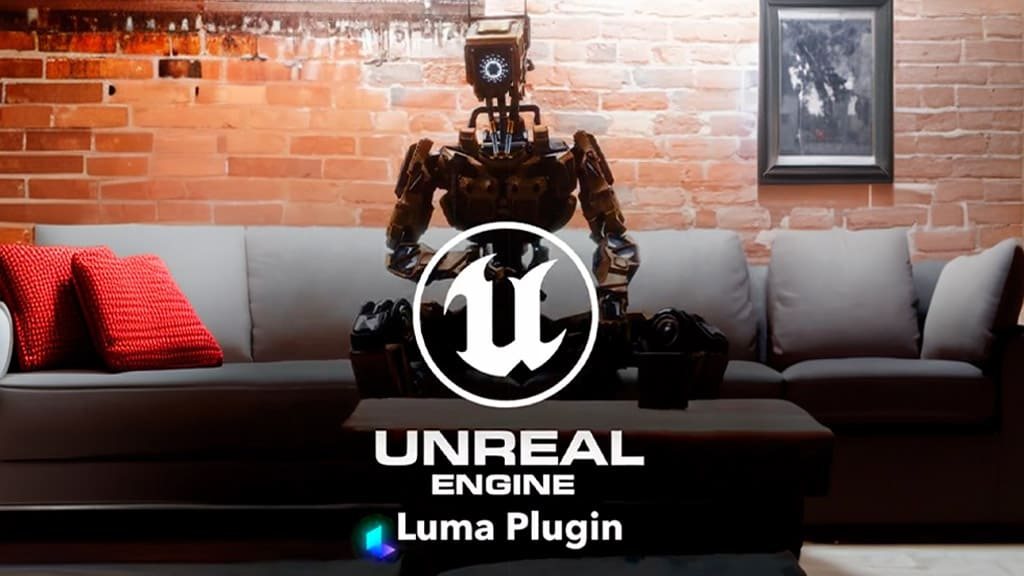
\includegraphics[scale=0.35]{./Figure/画像21.jpg}
  \caption{Unreal Engine 5 and Luma AI integration}
  \label{fig:Unreal Engine 5 and Luma AI integration}
\end{figure}
\begin{figure}[htbp]
  \centering
  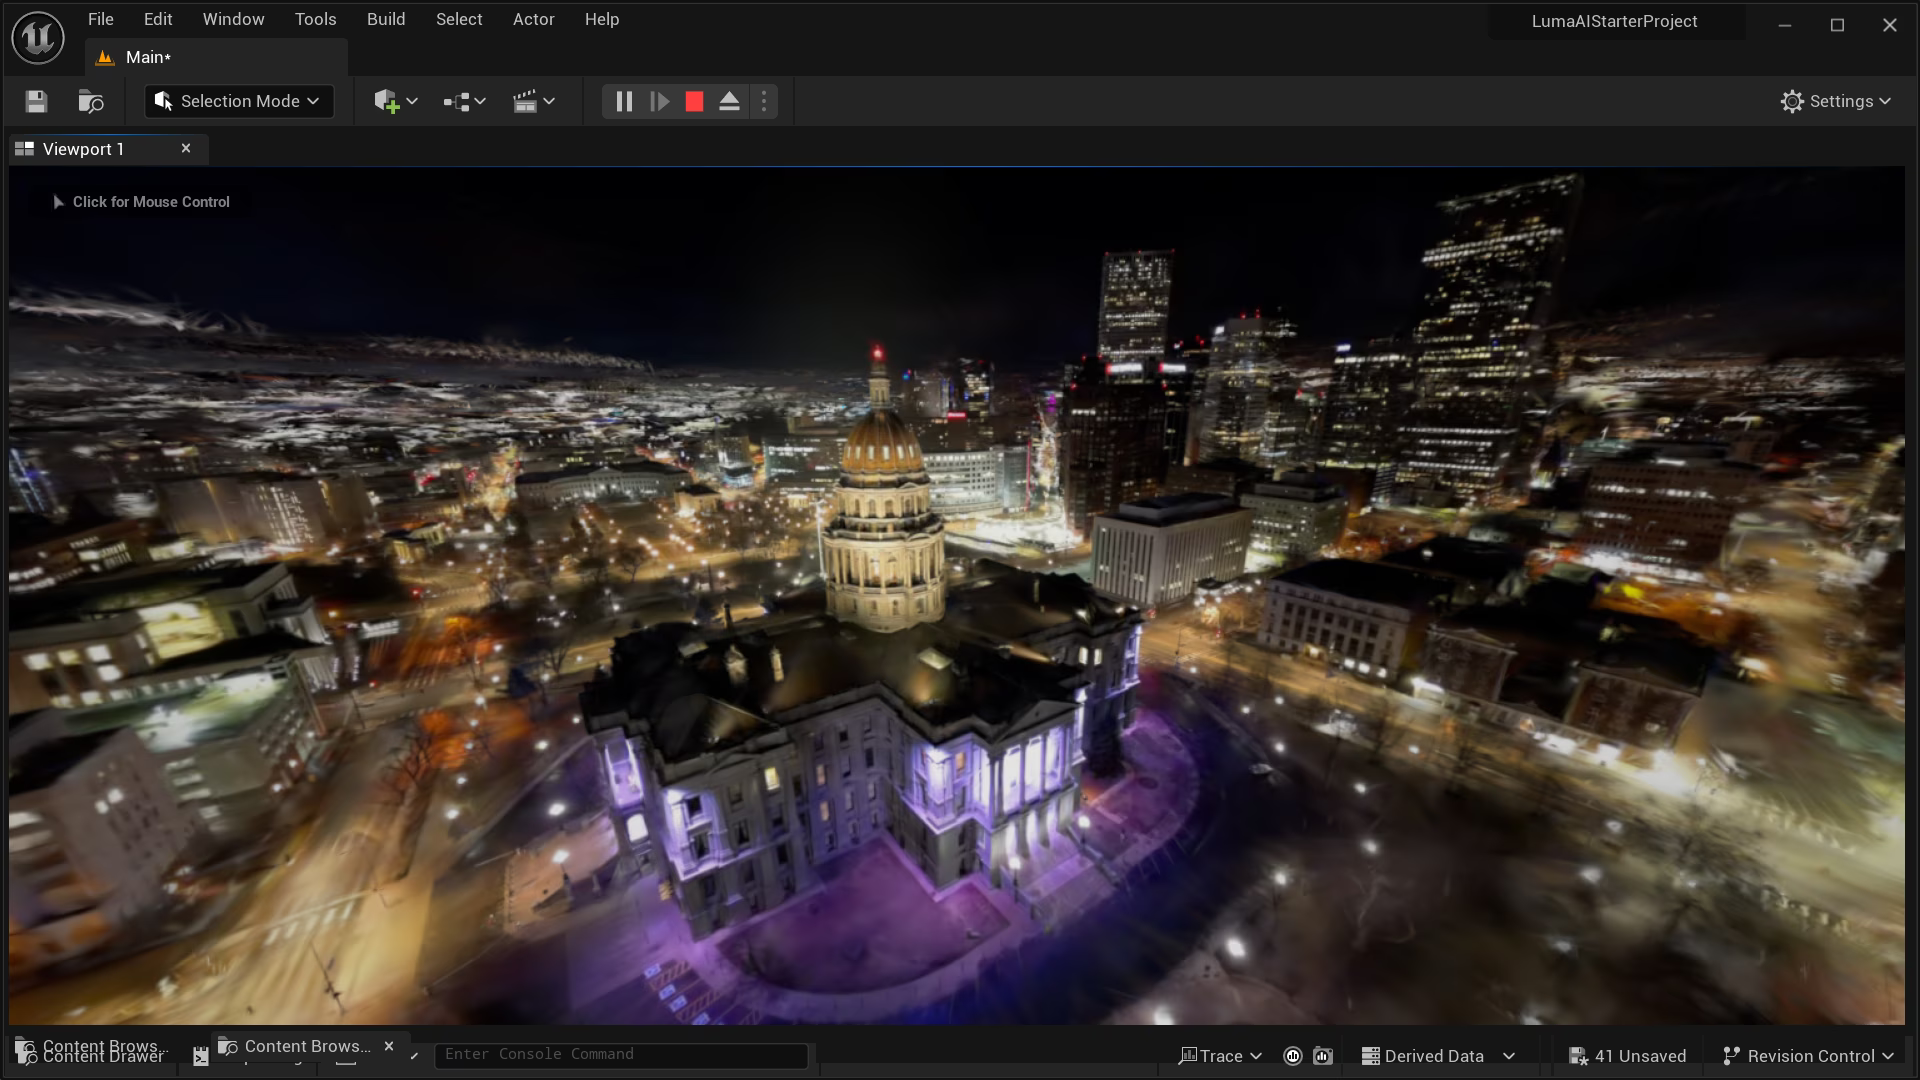
\includegraphics[scale=0.2]{./Figure/ppp.png}
  \caption{Unreal Engine 5 and Luma AI integration presents 3D virtual enviroment in Unreal engine5}
  \label{fig:Unreal Engine 5 and Luma AI integration presents 3D virtual enviroment in Unreal engine5}
\end{figure}

\section{3D Photorealistic Environment in Unreal Engine 5}
\label{sec:3D Photorealistic Environment in Unreal Engine 5}
\singlespacing
The process of integrating Luma AI and Unreal Engine 5 (UE5) is a significant aspect in the realm of advanced computer graphics and AI-driven applications\cite{luma2023unreal}(see Fig.\ref{fig:Unreal Engine 5 and Luma AI integration}, \ref{fig:Unreal Engine 5 and Luma AI integration presents 3D virtual enviroment in Unreal engine5}). It commences by obtaining data processed by Luma AI, usually obtainable for download from the Luma AI website in the .luma format. These .luma files contain the data processed by Luma AI and constitute a pivotal junction of AI processing and graphical rendering.
\singlespacing
The next step is to import the .luma files into UE5. This is done by placing them within Unreal Engine 5's content management system. The data processed by Luma AI is then integrated directly into UE5. This allows users to take advantage of UE5's advanced rendering and simulation capabilities, enhanced by the AI-driven data from Luma AI. This collaboration showcases the synergy between AI processing and real-time rendering, leading to enhanced and lifelike simulations in virtual environments.
\singlespacing
\begin{figure}[htbp]
  \centering
  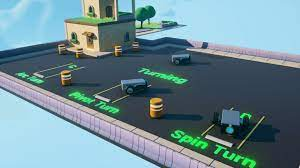
\includegraphics[scale=1]{./Figure/robot_in_unreal_engine.jpg}
  \caption{robot in Unreal engine5}
  \label{fig:robot in Unreal engine5}
\end{figure}
\subsection{Unreal Engine 5}
\label{sec:Unreal Engine 5}
\singlespacing
Unreal Engine 5 (UE5) \cite{unreal2023engine}is a game engine developed by Epic Games. It is the successor to Unreal Engine 4, which was released in 2014. The engine was first announced in March 2018 and was released in early access on May 13, 2021. The engine is designed for use in video games, but it can also be used for other applications such as virtual reality, augmented reality, and architectural visualization. Unreal engine 5 are used in robotics (see Fig.\ref{fig:robot in Unreal engine5})
\singlespacing
At the heart of Unreal Engine 5 lies its revolutionary rendering architecture, designed to deliver photorealistic visuals and dynamic global illumination in real-time. This is primarily facilitated by two core technologies: Nanite and Lumen. Nanite is a virtualized geometry technology that allows artists to create as much geometric detail as the eye can see. This virtualized micropolygon geometry frees creators from polygon budget constraints and the often tedious and time-consuming task of baking details into normal maps. With Nanite, users can import film-quality source art comprising hundreds of millions or billions of polygons directly into Unreal Engine, and it will be streamed and scaled in real time with no loss in quality.
\singlespacing
Lumen, on the other hand, is a fully dynamic global illumination solution that reacts immediately to scene and light changes, accurately simulating the subtle and complex interplays of light and shadow in an environment. With Lumen, artists and designers can create more dynamic scenes, where indirect lighting adapts on the fly to changes to direct lighting or geometry, such as changing the sun's angle with the time of day, turning on a flashlight, or opening an exterior door. This leads to a significant reduction in the time required to tweak lighting scenarios and settings, enabling a more intuitive design process.
\singlespacing
Another major feature of Unreal Engine 5 is its enhanced support for open worlds and large-scale environments. This is achieved through a new World Partition system, which changes how levels are managed and streamed, automatically dividing the world into a grid and streaming the necessary cells. This system makes it easier for teams of any size to collaborate on massive worlds without running into the typical bottlenecks associated with such large-scale projects.
\singlespacing
Unreal Engine 5 also introduces significant improvements in animation and physics. The engine integrates a new animation toolset that facilitates more dynamic and realistic movements and interactions. The advancements in physics simulation, along with the introduction of the Niagara VFX system, allow for more detailed and interactive environments. These features are essential for creating immersive experiences in games and simulations, where realism and responsiveness are key.
\singlespacing
Furthermore, UE5 includes robust audio tools like MetaSounds, a high-performance system that provides complete control over audio DSP graph generation of sound sources, leading to richer, more dynamic auditory environments. This level of control enables sound designers to create more complex and dynamic auditory experiences that can adapt in real time to the game or scene's events.
\singlespacing
In terms of usability, Unreal Engine 5 has been designed with a focus on making it more accessible and user-friendly, without sacrificing the depth and complexity that experienced developers expect. The user interface has been refined, and new features like the UI of Quixel Bridge have been integrated directly into the engine, streamlining the workflow for accessing a vast library of high-quality assets.
\singlespacing
In conclusion, Unreal Engine 5 represents a quantum leap in game engine technology, offering groundbreaking innovations in graphics rendering, world-building, animation, physics, and audio. Its suite of tools and features positions it as a key enabler for the next generation of real-time 3D content, pushing the boundaries of what is possible in game development, film production, architectural visualization, and beyond. Its focus on scalability, performance, and quality makes it a versatile choice for developers and creators aiming to craft experiences that are both visually stunning and deeply immersive.



\begin{figure}[htbp]
  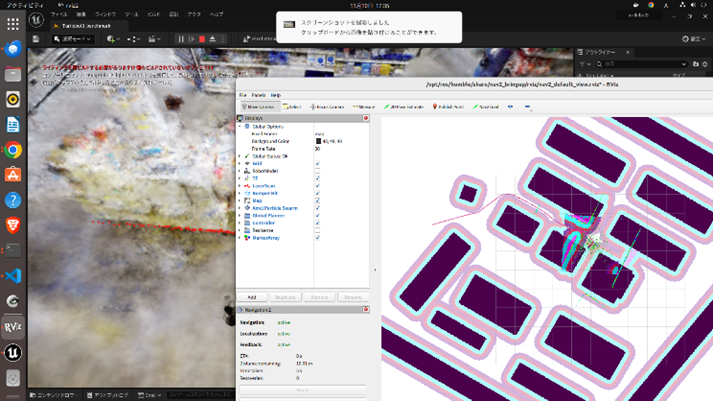
\includegraphics[scale=1.8]{./Figure/画像17.png}
  \caption{We navigated Turtlebot3 by navigation2  in Unreal Engine 5}
  \label{fig:We navigated Turtlebot3 by navigation2  in Unreal Engine 5}
\end{figure}

\section{Deployment of Turtlebot3 Robot in Virtual Environments}
\label{sec:Deployment of Turtlebot3 Robot in Virtual  Environments}
\singlespacing
The deployment of the Turtlebot3, specifically the waffle model, provides an intriguing case study in real and virtual robotic environments. Unreal Engine 5 (UE5) is used as the simulation platform in the virtual environment, and integrating the Turtlebot3 waffle with UE5 is accomplished using rcIUE\cite{rapyuta2023rclue}in conjunction with ROS2 Humble. This configuration enables the utilisation of sophisticated robotic features like Navigation2 and Simultaneous Localization and Mapping (SLAM). UE5's deployment enables thorough testing and enhancement of the robot's abilities through an extensive and lifelike simulation platform, unbound by any physical limitations.
\singlespacing
To operate in the actual environment(see.Fig.\ref{fig:We navigated Turtlebot3 by navigation2  in Unreal Engine 5}), we use the same Turtlebot3 waffle model, which is directed using ROS2 Humble. Directly controlling the robot in a physical setting enables practical implementation and testing, providing valuable insights into its performance and adaptability in real-world scenarios. The transition from virtual to physical environments highlights the versatility of the Turtlebot3 Waffle and its compatibility with ROS2 Humble, demonstrating its potential for diverse applications in the field of robotics.
\singlespacing
\section{Virtual Environment Evaluation}
\label{sec:Virtual Environment Evaluation}
\singlespacing
For the evaluation of our robotic simulation environment, we used Navigation2 to assess operational efficacy in a virtual setting, achieving a high success rate. We also integrated object recognition capabilities using You Only Look Once (YOLO). Specifically, we used a pre-trained YOLOX\cite{ge2021yolox} model. This study focused on recognizing objects in both real and virtual environments, with a particular emphasis on identifying identical objects across these settings. The effectiveness of cross-environment object recognition was quantitatively measured using the F1 score. We conducted a comprehensive analysis comparing the time and resources required to create virtual environments using our approach with those required for other studies such as NeRF2Real\cite{byravan2023nerf2real} and Matterport3D\cite{chang2017matterport3d}. The analysis focused on aspects such as computational efficiency and the need for specialized expertise. This comparison provided valuable insights into the relative performance and efficiency of our approach within the broader context of robotic simulation research.
\singlespacing
The F1 score is calculated as:
\begin{equation}
  precision = \frac{TP}{TP + FP}
\end{equation}
  
\begin{equation}
  recall = \frac{TP}{TP + FN}
\end{equation}

\begin{equation}
  F1-score = 2 \times \frac{precision \times recall}{precision + recall}
\end{equation}
\singlespacing
Here, TP (True Positives) is the count of objects correctly recognized as the same in both real and virtual environments, and FP (False Positives) is the count of objects that are incorrectly recognized as the same. FN (False Negatives) is the count of objects that are actually the same in both environments but were not recognized as such.

\subsection{YoloX}
\label{sec:You Only Look Once(Yolo)X}
\singlespacing
YOLOX\cite{ge2021yolox} represents the cutting-edge in real-time object detection within the realm of deep learning algorithms. As an evolution of the YOLO (You Only Look Once) series, YOLOX distinguishes itself by its ability to detect objects in an image through a singular inference process. This contrasts sharply with traditional object detection systems, which typically require a two-stage process involving region proposal and classification. YOLOX, however, amalgamates these tasks, achieving both simultaneously in one fell swoop.
\singlespacing
\begin{figure}[htbp]
  \centering
  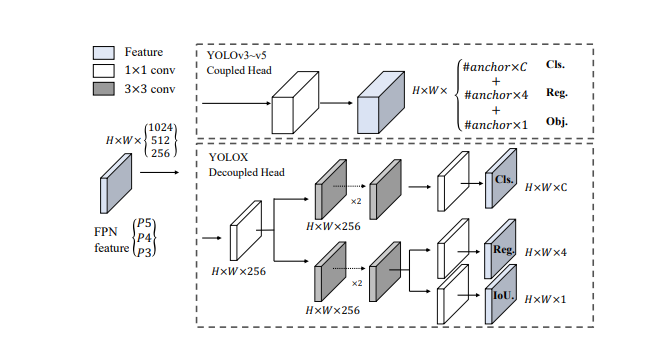
\includegraphics[scale=0.6]{./Figure/画像22.png}
  \caption{Illustration of the difference between YOLOv3 head and the proposed decoupled head.}
  \label{fig: Illustration of the difference between YOLOv3 head and the proposed decoupled head.}
\end{figure}
\singlespacing
The architecture of YOLOX is a tripartite structure, comprising a backbone, a neck, and a head. Each component plays a pivotal role: the backbone extracts features from images, the neck refines these features, and the head is responsible for the final object detection and classification.


\subsubsection{Backbone}
\label{sec:Backbone}
\singlespacing
The backbone typically employs efficient convolutional networks, such as Darknet or CSPDarknet. These networks are adept at extracting salient features from images with high efficiency.

\subsubsection{Neck}
\label{sec:Neck}
\singlespacing
The neck utilizes structures like Feature Pyramid Networks (FPN) or Path Aggregation Networks (PAN) to integrate features across different scales. This integration enhances the detection capabilities for objects of varying sizes, from the diminutive to the substantial.

\subsubsection{Head}
\label{sec:Head}
\singlespacing
In the head segment, bounding box prediction and class classification occur. YOLOX adopts an anchor-free approach, which, compared to traditional anchor-based methods, offers more flexibility and efficiency in object detection.



The core of YOLOX's functionality can be described through its loss function, which is a combination of coordinate loss, objectness loss, and class classification loss.
\singlespacing
\begin{align}
\text{Loss Function} = & \ \lambda_{\text{coord}} \times \text{Coordinate Loss} \nonumber \\
                      & + \lambda_{\text{obj}} \times \text{Objectness Loss} \nonumber \\
                      & + \lambda_{\text{cls}} \times \text{Class Classification Loss}
\label{equ:Loss Function}
\end{align}

Where $\lambda_{\text{coord}}$, $\lambda_{\text{obj}}$, and $\lambda_{\text{cls}}$ are the weights for the respective losses.

\subsubsection{Coordinate Loss}
\singlespacing
Coordinate loss measures the discrepancy between predicted and actual bounding boxes, often using an IoU-based loss.

\subsubsection{Objectness Loss}
\singlespacing
Objectness loss assesses the error in predicting the presence of an object, typically employing binary cross-entropy loss.

\subsubsection{Class Classification Loss}
\singlespacing
Class classification loss evaluates the error between predicted and actual classes, using cross-entropy loss.
\singlespacing
YOLOX is a powerful tool in real-time object detection, offering a blend of speed and accuracy. Its ongoing development is expected to continue pushing the boundaries in the field of computer vision.


\chapter{Experiment Result}
\label{chap:ExperimentResult}

\section{Comparison of Computational Efficiency and Resource Usage}
\label{sec:ComparisonofComputationalEfficiencyandResourceUsage}
\begin{table*}[htbp]
    \caption{Comparison of Computational Efficiency and Resource Usage}
    \centering
    \begin{tabularx}{\textwidth}{|X|X|X|X|}
        \hline
        Method & Means of Photography & Environment Creation Time (from images) & Need for specialized expertise \\
        \hline
        NeRF2Real [5] & Smartphone camera & 2-3 hours & Yes \\
        \hline
        Matterport3D [6] & Camera rig & Several days & Yes \\
        \hline
        Our method & Smartphone camera & 1-2 hours & No \\
        \hline
    \end{tabularx}
    \label{tab:ComparisonofComputationalEfficiencyandResourceUsage}
\end{table*}

\singlespacing
The Table.\ref{tab:ComparisonofComputationalEfficiencyandResourceUsage} elucidated in the table underscores pronounced disparities in computational efficiency and resource utilization across three paradigms for virtual environment creation: NeRF2Real, Matterport3D, and Our Method. Each paradigm employs distinct photographic techniques and varies in temporal commitments for environment genesis, alongside requisites for specialized acumen. 
\singlespacing
NeRF2Real, deploying a smartphone camera, strikes a nuanced equilibrium between alacrity and technical intricacy. It necessitates roughly 2-3 hours for creating an environment, apt for compact spaces. Nonetheless, the prerequisite of eight NVIDIA V100 GPUs and specialized knowledge renders it less attainable for the layperson. This method is propitious for scenarios seeking a harmonious blend of efficacy and professional caliber, yet its dependence on advanced GPUs and technical prowess curtails its widespread applicability.
\singlespacing
Conversely, Matterport3D markedly prolongs the environmental creation process, spanning several days. Predicated on a camera rig, it demands not only specialized apparatus but also expert intervention. Its protracted creation interval and need for specialized rigging augment the precision and intricacy of the resultant environments, rendering it exemplary for professional-grade simulations. However, its complexity and resource exigencies render it impracticable for casual or resource-constrained entities.
\singlespacing
Our method distinguishes itself as the most user-centric and accessible alternative. Leveraging a smartphone camera, it requires a mere 1-2 hours for environment creation, eschewing the need for specialized expertise. This method democratizes virtual environment creation, rendering it attainable for individuals devoid of technical backgrounds or significant resources. Its simplicity and cost-efficiency designate it as the quintessential choice for casual users or those desiring a straightforward pathway to environment simulation.
\singlespacing
In summation, juxtaposing these tripartite methodologies unveils a spectrum of options for virtual environment creation, each catering to divergent requisites and resource availabilities. NeRF2Real presents a median path with moderate efficiency and complexity; Matterport3D offers high-fidelity environments at the expense of substantial resources; and Our method emerges as the most accessible and user-friendly, accommodating an expansive array of users.



\section{Yolo Result}
\label{sec:YoloResult}

\begin{table*}[htbp]
    \caption{Comparison of Object Recognition Performance in Real and Virtual Environments}
    \centering
    \begin{tabularx}{\textwidth}{|X|X|X|X|X|}
        \hline
        Environment & TP & FP & FP & F1-score \\
        \hline
        Kiosk & 2 & 1 & 0 & 80\% \\
        \hline
        Research Building & 5 & 0 & 0 & 100\% \\
        \hline
    \end{tabularx}
    \label{tab:ComparisonofObjectRecognitionPerformanceinRealandVirtualEnvironments}
\end{table*}
\begin{figure}[htbp]
  \centering
  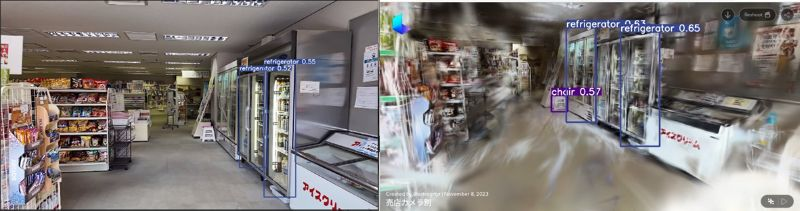
\includegraphics[scale=0.5]{./Figure/Object Recognition at the University of Aizu Kios}
  \caption{Object Recognition at the University of Aizu Kios}
  \label{fig: Object Recognition at the University of Aizu Kios}
\end{figure}
This study compared the performance of object recognition models in real-world and virtual environments and evaluated the agreement rate between these settings. This analysis shows that the match rate is over 80\%, indicating that the virtual environment effectively reflects the real-world scenario. Specifically, the object recognition models showed different performance in different environments. In the kiosk environment, the model had two true positives (TP), one false positive (FP), no false negatives (FN), and an F1 score of 80\%. In contrast, in a lab environment, the model achieved a perfect F1 score of 100\% with 5 true positives and no false positives or negatives. These results suggest that the performance of object detection models varies greatly depending on the environment, and is particularly influenced by the complexity of the setting and the diversity of objects present. This paragraph compares the performance of object recognition models in real-world and virtual environments and highlights the variation in performance in different environments(see Fig.\ref{fig: Object Recognition at the University of Aizu Kios}).
\singlespacing
In addition, we have included the results of YOLO (You Only Look Once) object detection in \ref{tab:ComparisonofObjectRecognitionPerformanceinRealandVirtualEnvironments}. This inclusion provides a comprehensive view of the effectiveness of different models in object detection tasks within these environments. The YOLO model's results further validate our findings and offer an in-depth perspective on the capabilities and limitations of current object detection technologies. This study provides crucial insights supporting the virtual environment's adequacy in accurately replicating the complexities of real-world settings and its validity as a simulation tool in the field of robotics.
\begin{figure}[htbp]
  \centering
  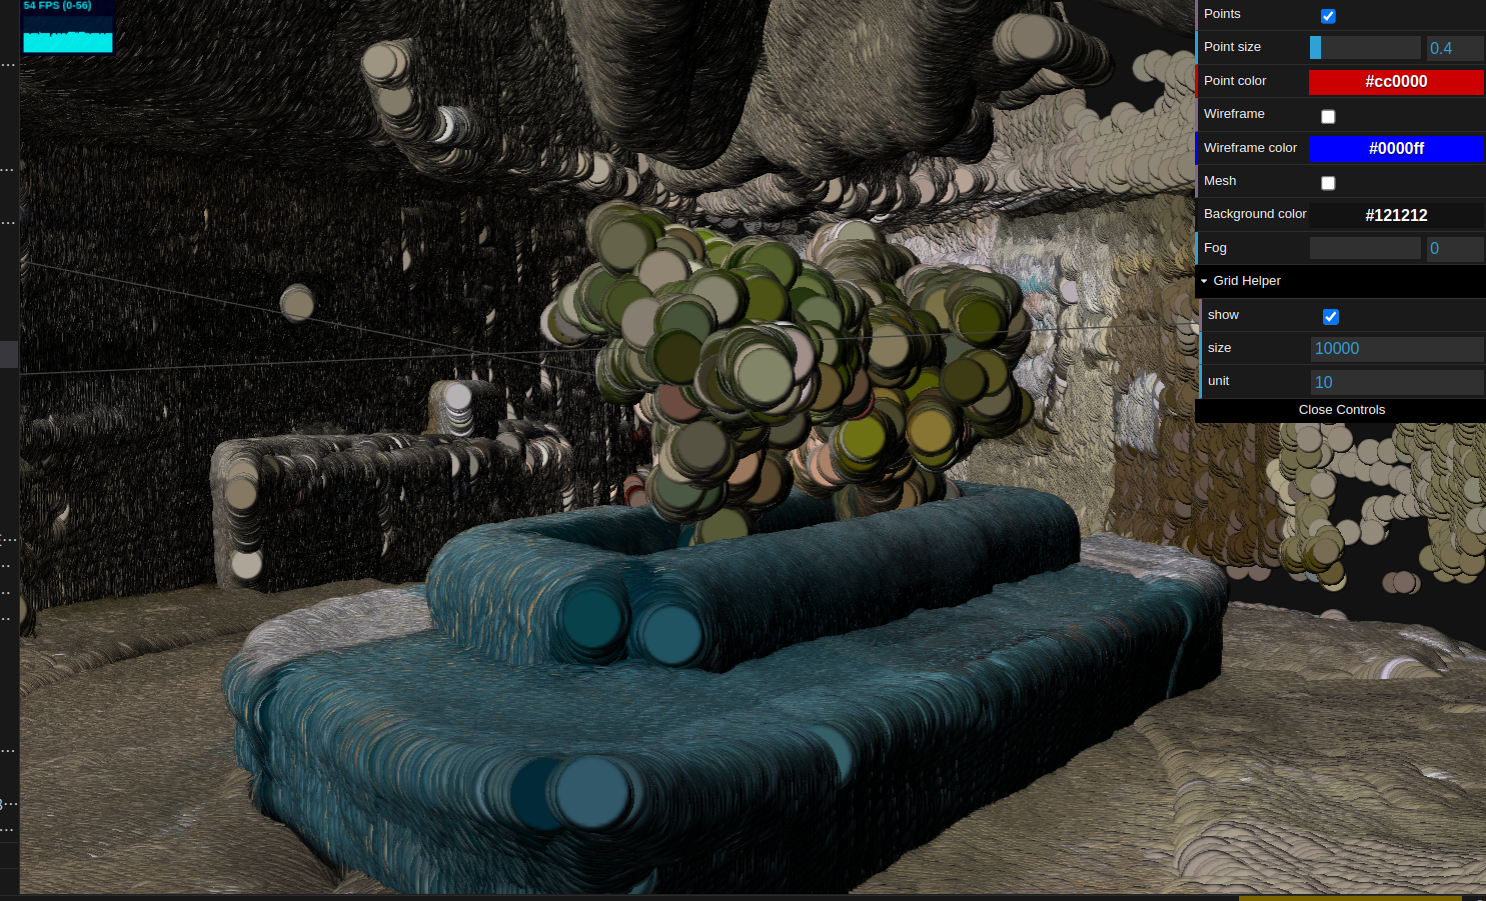
\includegraphics[scale=0.3]{./Figure/研究等の点群.png}
  \caption{Point cloud of the research building generated by Luma AI}
  \label{fig: Point cloud of the research building generated by Luma AI}
\end{figure}
\
\begin{figure}[htbp]
  \centering
  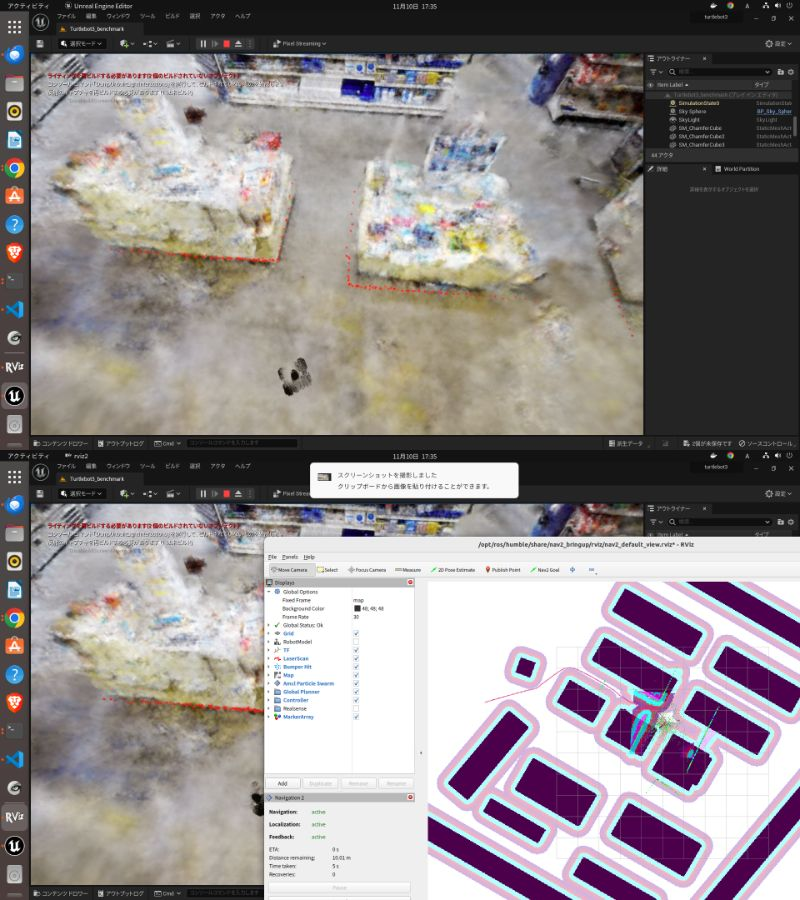
\includegraphics[scale=0.5]{./Figure/n.jpg}
  \caption{Navigation through physical phenomena using point clouds and 3D environments}
  \label{fig:Navigation through physical phenomena using point clouds and 3D environments}
\end{figure}
\section{Navigation2 Result}
\label{sec:Navigation2Result}
This research explores the potential of navigation technology in virtual environments. In particular, focusing on Navigation 2, we combined the point cloud data generated by LumaAI (see. fig\ref{fig: Point cloud of the research building generated by Luma AI}) and Unreal Engine 5's lidar plugin\cite{unrealengine_lidar_plugin} to realize the physical settings of the object. Using this technology, the turtlebot3 waffle model successfully simulated navigation within a virtual environment. This research result represents a major advance in the development of navigation systems in virtual environments.


\chapter{Discussion}
\label{chap:discussion}

\section{Virtual Environment Creation}
\label{sec:Virtual Environment Creation}
The results pertaining to virtual environment creation (Section \ref{sec:ComparisonofComputationalEfficiencyandResourceUsage}) underscore a significant disparity in the balance between ease of use, resource requirements, and technical expertise among the compared methods. It is evident that while methods like NeRF2Real and Matterport3D offer high precision and quality in environment creation, they necessitate substantial technical expertise and resources, thus limiting their accessibility to specialists and well-equipped organizations. In contrast, Our Method, with its minimal resource requirement and elimination of the need for specialized expertise, democratizes the process of virtual environment creation. This accessibility suggests a potential shift in the field towards more user-friendly and resource-efficient methodologies, particularly beneficial for individuals and smaller entities. The implications here are twofold: firstly, the democratization of virtual environment creation could lead to broader adoption and innovation in various fields, and secondly, it raises questions about the balance between quality and accessibility in technological advancements.

\section{Object Recognition Performance}
\label{sec:Object Recognition Performance}
The study of object recognition performance in real and virtual environments (Section \ref{sec:YoloResult}) reveals significant findings regarding the efficacy of virtual environments in replicating real-world scenarios. The high agreement rate of over 80\% in object recognition models across these environments suggests that virtual environments can effectively mirror the real world. However, the variation in performance, as observed in the kiosk and research building environments, indicates the influence of environmental complexity and object diversity on model accuracy. This underlines the importance of considering environmental factors when deploying object recognition models. The successful application of the YOLO model further validates the reliability of virtual environments in simulating real-world settings, which can have profound implications for the fields of robotics and AI training.

\section{Navigation Technology in Virtual Environments}
\label{sec:Navigation Technology in Virtual Environments}
The exploration of Navigation 2 technology, as discussed in Section \ref{sec:Navigation2Result}, represents a significant stride in the application of virtual environments for navigation system development. The successful simulation of navigation within a virtual environment using combined technologies from LumaAI and Unreal Engine 5 highlights the potential of virtual environments as a testing ground for developing and refining navigation technologies. This has crucial implications for areas such as robotics, autonomous vehicles, and AI, where real-world testing can be resource-intensive and potentially hazardous.

\section{Limitations and Future Directions}
\label{sec:Limitations and Future Directions}
While the study provides valuable insights, there are limitations that need to be addressed in future research. One major limitation is the scope of environments and models tested. Extending the research to include a broader range of environments and object recognition models would provide a more comprehensive understanding of the capabilities and limitations of virtual environments. Additionally, exploring the scalability of these technologies in more complex and dynamic real-world scenarios would provide further validation of their practicality and effectiveness.

This study contributes significantly to the understanding of virtual environment creation, object recognition in different settings, and navigation technologies. The findings suggest a shift towards more accessible and resource-efficient technologies in virtual environment creation, affirm the effectiveness of virtual environments in replicating real-world scenarios for object recognition, and highlight the potential of virtual settings in developing navigation technologies. However, future research addressing the noted limitations is essential to further advance the field.






\chapter{Conclusion}
\label{chap:conclusion}
This thesis presents a novel approach to creating photorealistic 3D virtual environments for robotics, leveraging the synergy between Luma AI’s Neural Radiance Fields (NeRF) and Unreal Engine 5 (UE5). The research successfully demonstrates a cost-effective and efficient pipeline for generating these environments using standard smartphone cameras, significantly reducing the time and resources compared to existing methods like NeRF2real and Matterport3D. The practical application of this approach is evidenced by the deployment of the Turtlebot3 robot in these virtual environments, controlled via ROS2 Humble, and the achievement of high F1 scores in cross-environment object recognition. This methodology facilitates more effective simulation-driven development and testing in robotics, setting a new standard for virtual environment generation. However, the reliance on Luma AI as a sole processing platform is identified as a potential limitation, indicating a direction for future research towards developing independent or alternative platforms. The thesis contributes significantly to the field of robotic simulation, offering a practical solution to the challenges of creating and utilizing photorealistic 3D environments in robotics.







% % %
% End of Body
% % %

% % Bibliography style
\singlespacing
\bibliographystyle{IEEEtran}
\bibliography{ref}
% % Bibliography style


% % If you add references to a table of contents, uncomment the following line
% \addcontentsline{toc}{chapter}{References}

% % You can make appendixes, if any.
% \appendix
% \include{./Chapter/hogehoge.tex}

\end{document}
